\section{Inside FlashAttention}
\begin{frame}{}
    \LARGE \textbf{Inside FlashAttention}
\end{frame}

\begin{frame}{Why Fast Attention Is a Memory Problem}
    \begin{columns}[T,onlytextwidth]
        \column{0.50\textwidth}
        \begin{itemize}\itemsep0.5em
            \item Transformer training is usually \textbf{memory-bound}: matrix multiplications account for 99.8\% of the FLOPs but only 61\% of the runtime.
            \item Nearly 40\% of the time goes to softmax, dropout, masking, and normalization --- operations that do almost no arithmetic but stream whole tensors through GPU memory.
            \item Recall the hierarchy from the FlashAttention-2 discussion: roughly 20\,MB of on-chip SRAM at 19\,TB/s against 40--80\,GB of HBM at 1.5--2\,TB/s.
            \item So the lever for faster attention is not fewer FLOPs; it is \textbf{less data movement}.
        \end{itemize}
        \column{0.47\textwidth}
        \centering
        \vspace{1.5em}
        {\footnotesize
        \begin{tabular}{lrr}
            \toprule
            Operator class & \% FLOPs & \% runtime \\
            \midrule
            Tensor contraction & 99.80 & 61.0 \\
            Stat.\ normalization & 0.17 & 25.5 \\
            Element-wise & 0.03 & 13.5 \\
            \bottomrule
        \end{tabular}}\\[0.8em]
        {\scriptsize Operator classes in a PyTorch BERT training step. Ivanov et al., ``Data Movement Is All You Need: A Case Study on Optimizing Transformers,'' \href{https://arxiv.org/abs/2007.00072}{arXiv:2007.00072}, Table~1.}
    \end{columns}
\end{frame}

\begin{frame}{What Standard Attention Streams Through HBM}
    The textbook implementation materializes two $N \times N$ matrices in slow memory:
    \begin{enumerate}\itemsep0.4em
        \item Load $Q, K$ by blocks from HBM, compute $S = QK^\top$, \textbf{write $S$ to HBM}.
        \item Read $S$ from HBM, compute $P = \mathrm{softmax}(S)$, \textbf{write $P$ to HBM}.
        \item Load $P$ and $V$ by blocks from HBM, compute $O = PV$, write $O$ to HBM.
    \end{enumerate}
    \vspace{0.5em}
    \begin{itemize}\itemsep0.4em
        \item At $N = 4096$ in fp16, one head's score matrix is already $4096^2 \times 2\,\text{B} = 32$\,MiB --- larger than \emph{all} the SRAM on the GPU --- while the $Q$ tile it came from is half a MiB.
        \item Every step is a separate kernel: the $N \times N$ traffic is paid twice for $S$ and twice more for $P$, and again during the backward pass, which needs both matrices.
    \end{itemize}
    \vspace{0.5em}
    {\scriptsize Standard attention implementation, Algorithm~0 of Dao et al., ``FlashAttention: Fast and Memory-Efficient Exact Attention with IO-Awareness,'' \href{https://arxiv.org/abs/2205.14135}{arXiv:2205.14135}.}
\end{frame}

\begin{frame}{Tiling: The Oldest Trick in Fast Linear Algebra}
    Split the matrices into blocks; each output block is a short sum of block products:
    \[
        C =
        \begin{bmatrix}
            C_{00} & C_{01} \\
            C_{10} & C_{11}
        \end{bmatrix},
        \qquad
        C_{ij} = \sum_{k} A_{ik} B_{kj},
        \qquad
        C_{00} = A_{00}B_{00} + A_{01}B_{10} + A_{02}B_{20}.
    \]
    \begin{itemize}\itemsep0.3em
        \item With three tile-sized registers $X, Y, Z$ in fast memory, $C_{00}$ never leaves the chip until it is finished:
    \end{itemize}
    \vspace{-0.5em}
    \[
        \begin{aligned}
            X &\leftarrow A_{00}, & Y &\leftarrow B_{00}, & Z &\leftarrow XY, \\
            X &\leftarrow A_{01}, & Y &\leftarrow B_{10}, & Z &\leftarrow Z + XY, \\
            X &\leftarrow A_{02}, & Y &\leftarrow B_{20}, & Z &\leftarrow Z + XY, & C_{00} &\leftarrow Z.
        \end{aligned}
    \]
    \vspace{-0.5em}
    \begin{itemize}\itemsep0.3em
        \item Each input tile is read once per output block, and the big matrices live in slow memory only.
        \item The trick works because \textbf{addition is associative}: partial products can be accumulated in any order, one pair of tiles at a time. Every fast GEMM library is built on this.
    \end{itemize}
\end{frame}

\begin{frame}{Why Attention Resists Tiling}
    \[
        X' = \mathrm{softmax}\!\left(QK^\top / \sqrt{d_k}\right) V
    \]
    \begin{itemize}\itemsep0.5em
        \item The matrix products in attention tile perfectly --- but between them sits a row-wise softmax, and \textbf{softmax is not associative}.
        \item Each output row needs the row's \emph{global} maximum and normalizer:
        \[
            y_i = \frac{e^{x_i - m}}{\sum_{j=1}^{N} e^{x_j - m}},
            \qquad m = \max_k x_k,
        \]
        so no block of the output can be finalized until every block of the row has been seen.
        \item Tile the two matmuls naively and the softmax in the middle still forces the full $N \times N$ score matrix out to HBM --- which is exactly the traffic tiling was meant to remove.
    \end{itemize}
\end{frame}

\begin{frame}{Safe Softmax: Three Passes Over the Data}
    \begin{itemize}\itemsep0.4em
        \item The naive form $y_i = e^{x_i} / \sum_j e^{x_j}$ overflows quickly: $e^{89}$ exceeds the fp32 range, and $e^{12}$ already exceeds fp16.
        \item Every deep-learning library therefore computes the \textbf{safe softmax}, shifted by the maximum:
    \end{itemize}
    \begin{align*}
        \text{pass 1:}\quad & m = \max_k x_k \\
        \text{pass 2:}\quad & d = \textstyle\sum_{j=1}^{V} e^{x_j - m} \\
        \text{pass 3:}\quad & y_i = e^{x_i - m} / d
    \end{align*}
    \begin{itemize}\itemsep0.4em
        \item Numerically robust --- but it makes \textbf{three full passes} over the logits, and for large inputs each pass is a full trip through memory.
    \end{itemize}
    \vspace{0.3em}
    {\scriptsize Milakov \& Gimelshein, ``Online normalizer calculation for softmax,'' \href{https://arxiv.org/abs/1805.02867}{arXiv:1805.02867}, Algorithms~1--2.}
\end{frame}

\begin{frame}{Online Softmax: Two Passes}
    \begin{itemize}\itemsep0.4em
        \item The running maximum and the running normalizer can be maintained \textbf{in the same pass}. When a new element $x_j$ arrives:
    \end{itemize}
    \begin{align*}
        m_j &= \max(m_{j-1},\, x_j) \\
        d_j &= d_{j-1}\, e^{\,m_{j-1} - m_j} + e^{\,x_j - m_j}
    \end{align*}
    \begin{itemize}\itemsep0.4em
        \item The factor $e^{\,m_{j-1} - m_j}$ \textbf{retroactively rescales} everything accumulated so far, as if the new maximum had been known from the start; after one pass, $y_i = e^{x_i - m_V} / d_V$ needs only one more.
        \item Three passes become two: a 1.33$\times$ saving on paper and about 1.3$\times$ in practice, purely from reduced memory traffic --- the arithmetic went \emph{up}.
        \item This recurrence, published as a softmax micro-optimization, turned out to be the missing piece that lets attention be tiled.
    \end{itemize}
    \vspace{0.3em}
    {\scriptsize Milakov \& Gimelshein, \href{https://arxiv.org/abs/1805.02867}{arXiv:1805.02867}, Algorithm~3.}
\end{frame}

\begin{frame}{Operator Fusion: Skip the Round Trips}
    \begin{columns}[T,onlytextwidth]
        \column{0.48\textwidth}
        \centering
        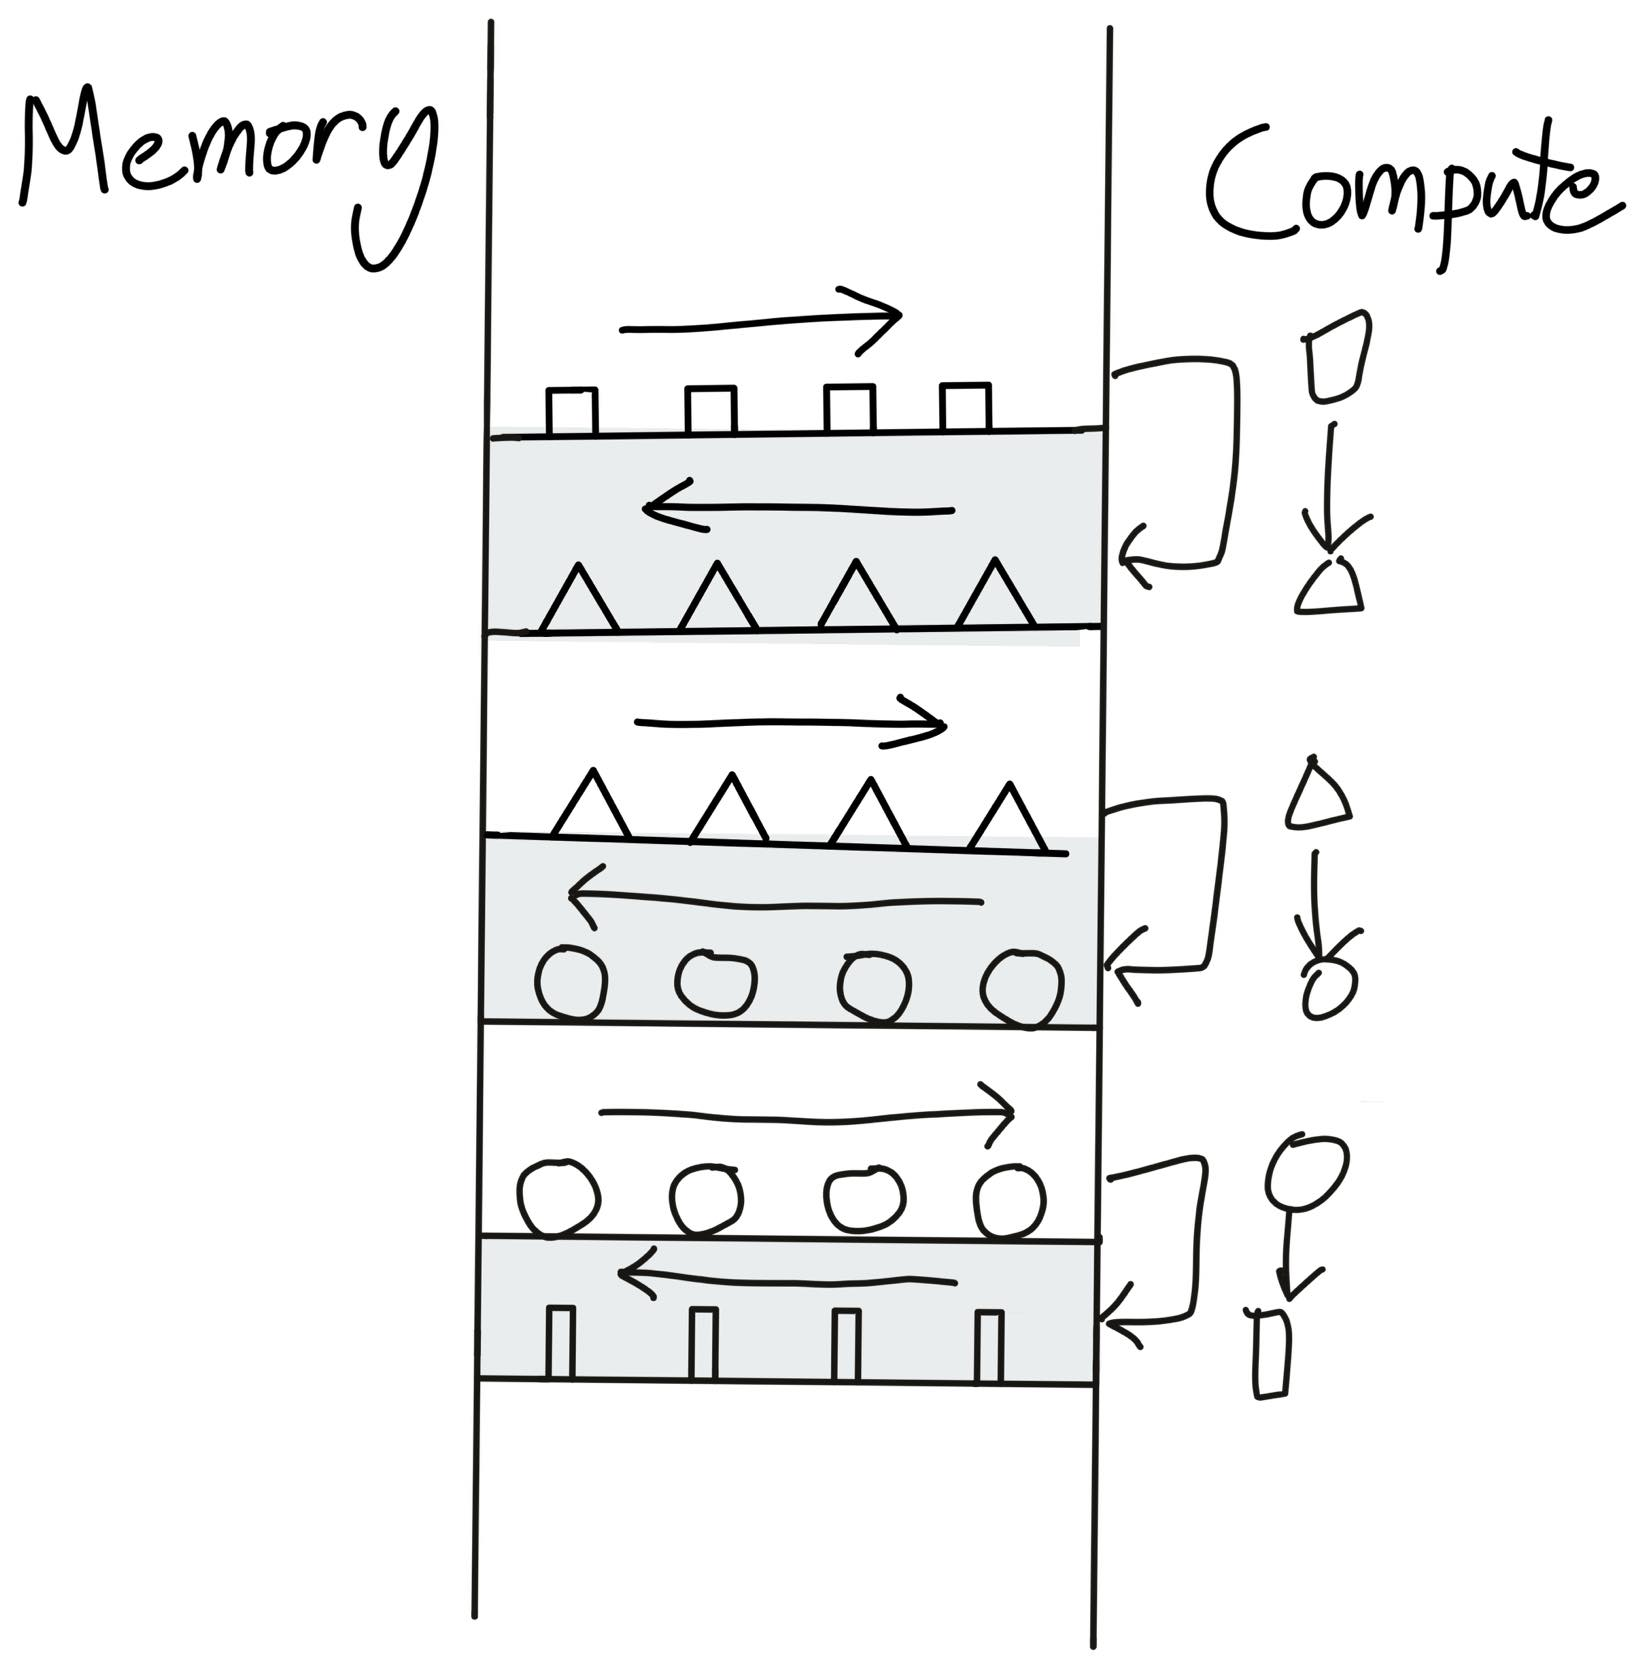
\includegraphics[width=0.66\linewidth,height=0.46\textheight,keepaspectratio]{images/recent-advance/horace-he-multi-operators.png}
        \column{0.48\textwidth}
        \centering
        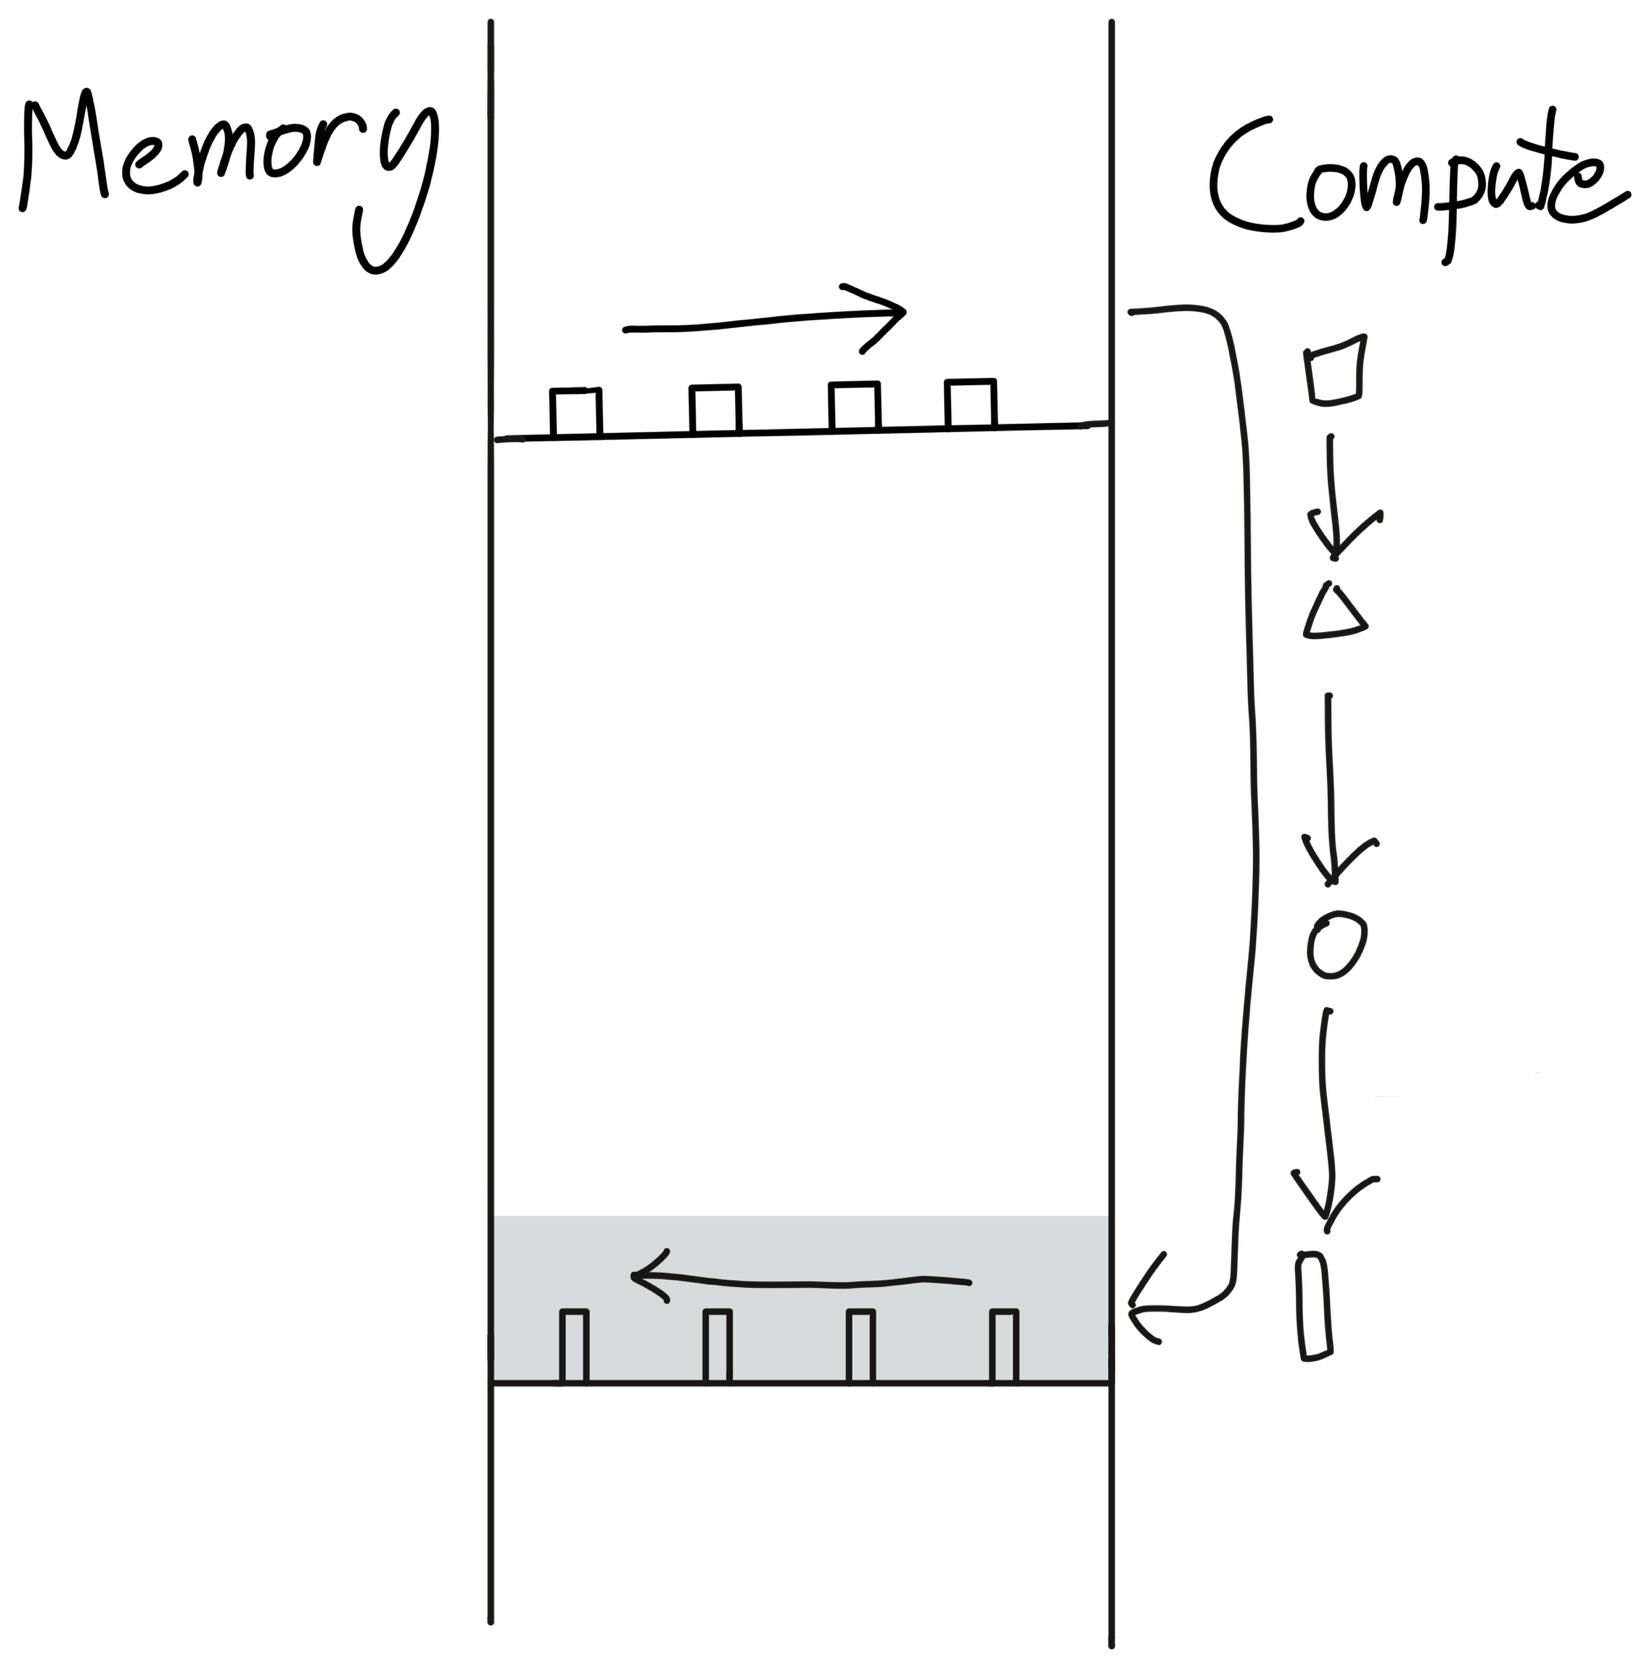
\includegraphics[width=0.66\linewidth,height=0.46\textheight,keepaspectratio]{images/recent-advance/horace-he-operator-fusion.png}
    \end{columns}
    \begin{itemize}\itemsep0.3em
        \item Unfused (left), every memory-bound op --- scale, mask, softmax, dropout --- pays its own HBM round trip; fused (right), the whole chain rides along in a single kernel in fast memory.
        \item Fusing \emph{across} attention's matmuls is exactly what the softmax normalizer forbids --- unless the softmax itself can be computed incrementally.
    \end{itemize}
    {\scriptsize Figures from Horace He, ``Making Deep Learning Go Brrrr From First Principles,'' \url{https://horace.io/brrr_intro.html}.}
\end{frame}

\begin{frame}{FlashAttention: Assembling the Pieces}
    Tile $K, V$ into blocks; keep running statistics $(m, \ell)$ and output $O$ per query row. For each incoming block $j$, compute on-chip
    \[
        S_j = QK_j^\top / \sqrt{d_k},
        \qquad
        m_j = \mathrm{rowmax}(S_j),
        \qquad
        P_j = e^{S_j - m_j},
        \qquad
        \ell_j = \mathrm{rowsum}(P_j),
    \]
    then fold it into the running answer with the online-softmax correction:
    \begin{align*}
        m' &= \max(m,\, m_j),
        \qquad
        \ell' = e^{\,m - m'}\,\ell + e^{\,m_j - m'}\,\ell_j, \\[0.2em]
        O' &= \frac{\ell\, e^{\,m - m'}}{\ell'}\, O \;+\; \frac{e^{\,m_j - m'}}{\ell'}\, P_j V_j.
    \end{align*}
    \begin{itemize}\itemsep0.3em
        \item This is the online-softmax recurrence upgraded from a running sum to a running \emph{weighted sum of value rows}: the $N \times N$ matrix is never materialized, and the result is \textbf{exact}.
        \item FlashAttention-2's ``fewer non-matmul FLOPs'' improvement is precisely a deferral of the division by $\ell$ to the very end of the loop.
    \end{itemize}
    \vspace{0.2em}
    {\scriptsize Dao et al., \href{https://arxiv.org/abs/2205.14135}{arXiv:2205.14135}, Algorithm~1 (lines 10--12); simplified to one query block.}
\end{frame}

\begin{frame}{Recomputation: Spending FLOPs to Save Memory}
    \begin{columns}[T,onlytextwidth]
        \column{0.55\textwidth}
        \begin{itemize}\itemsep0.5em
            \item The backward pass needs the attention matrices $S$ and $P$ --- but storing them would reintroduce the $N \times N$ traffic.
            \item FlashAttention stores only the output $O$ and the softmax statistics $(m, \ell)$, of size $N$, and \textbf{recomputes} the needed tiles of $S$ and $P$ on-chip during the backward pass.
            \item The result does \emph{more} arithmetic than standard attention, moves $9\times$ less data, and finishes almost $6\times$ sooner --- the memory-bound argument, closed in one table.
        \end{itemize}
        \column{0.42\textwidth}
        \centering
        \vspace{1.5em}
        {\small
        \begin{tabular}{lrr}
            \toprule
            & Standard & Flash \\
            \midrule
            GFLOPs & 66.6 & 75.2 \\
            HBM R/W (GB) & 40.3 & 4.4 \\
            Runtime (ms) & 41.7 & 7.3 \\
            \bottomrule
        \end{tabular}}\\[0.8em]
        {\scriptsize Forward + backward of one attention layer, GPT-2 medium on an A100. Dao et al., \href{https://arxiv.org/abs/2205.14135}{arXiv:2205.14135}, Figure~2.}
    \end{columns}
\end{frame}

\begin{frame}{What Exactness Buys, and Where This Leads}
    \begin{itemize}\itemsep0.4em
        \item \textbf{No approximation:} the model and its perplexity are unchanged; only time and memory move. GPT-2 medium trains in 6.9 days against 21.0 for the baseline implementation, at identical quality.
        \item \textbf{Linear memory:} the footprint grows with $N$ instead of $N^2$, which is what made 16k-token Path-X tractable --- the first Transformer to beat chance on it.
        \item \textbf{Hardware--software co-design:} the algorithm is reorganized around the memory hierarchy, and each GPU generation reshapes the kernel --- the engineering that FlashAttention-2 carries further (see the \emph{Transformers: 2017 vs 2026} lecture).
        \item \textbf{Long context as the payoff:} IO-efficient exact attention is the entry ticket to the 128k-token windows of models like LLaMA 3, and to the long interactive sessions that agentic workloads demand; the serving-side levers (KV caching, paging, speculative decoding) are covered in the \emph{Inference Optimisation} lecture.
    \end{itemize}
\end{frame}
